% Options for packages loaded elsewhere
\PassOptionsToPackage{unicode}{hyperref}
\PassOptionsToPackage{hyphens}{url}
%
\documentclass[
  11pt,
]{article}
\usepackage{amsmath,amssymb}
\usepackage[]{times}
\usepackage{ifxetex,ifluatex}
\ifnum 0\ifxetex 1\fi\ifluatex 1\fi=0 % if pdftex
  \usepackage[T1]{fontenc}
  \usepackage[utf8]{inputenc}
  \usepackage{textcomp} % provide euro and other symbols
\else % if luatex or xetex
  \usepackage{unicode-math}
  \defaultfontfeatures{Scale=MatchLowercase}
  \defaultfontfeatures[\rmfamily]{Ligatures=TeX,Scale=1}
\fi
% Use upquote if available, for straight quotes in verbatim environments
\IfFileExists{upquote.sty}{\usepackage{upquote}}{}
\IfFileExists{microtype.sty}{% use microtype if available
  \usepackage[]{microtype}
  \UseMicrotypeSet[protrusion]{basicmath} % disable protrusion for tt fonts
}{}
\makeatletter
\@ifundefined{KOMAClassName}{% if non-KOMA class
  \IfFileExists{parskip.sty}{%
    \usepackage{parskip}
  }{% else
    \setlength{\parindent}{0pt}
    \setlength{\parskip}{6pt plus 2pt minus 1pt}}
}{% if KOMA class
  \KOMAoptions{parskip=half}}
\makeatother
\usepackage{xcolor}
\IfFileExists{xurl.sty}{\usepackage{xurl}}{} % add URL line breaks if available
\IfFileExists{bookmark.sty}{\usepackage{bookmark}}{\usepackage{hyperref}}
\hypersetup{
  pdftitle={Data Analysis report using R The unsuccessful performance of the Los Angeles Lakers team},
  pdfauthor={Panayiotis Kattides},
  hidelinks,
  pdfcreator={LaTeX via pandoc}}
\urlstyle{same} % disable monospaced font for URLs
\usepackage[margin=1in]{geometry}
\usepackage{longtable,booktabs,array}
\usepackage{calc} % for calculating minipage widths
% Correct order of tables after \paragraph or \subparagraph
\usepackage{etoolbox}
\makeatletter
\patchcmd\longtable{\par}{\if@noskipsec\mbox{}\fi\par}{}{}
\makeatother
% Allow footnotes in longtable head/foot
\IfFileExists{footnotehyper.sty}{\usepackage{footnotehyper}}{\usepackage{footnote}}
\makesavenoteenv{longtable}
\usepackage{graphicx}
\makeatletter
\def\maxwidth{\ifdim\Gin@nat@width>\linewidth\linewidth\else\Gin@nat@width\fi}
\def\maxheight{\ifdim\Gin@nat@height>\textheight\textheight\else\Gin@nat@height\fi}
\makeatother
% Scale images if necessary, so that they will not overflow the page
% margins by default, and it is still possible to overwrite the defaults
% using explicit options in \includegraphics[width, height, ...]{}
\setkeys{Gin}{width=\maxwidth,height=\maxheight,keepaspectratio}
% Set default figure placement to htbp
\makeatletter
\def\fps@figure{htbp}
\makeatother
\setlength{\emergencystretch}{3em} % prevent overfull lines
\providecommand{\tightlist}{%
  \setlength{\itemsep}{0pt}\setlength{\parskip}{0pt}}
\setcounter{secnumdepth}{5}
\usepackage[labelfont={bf}]{caption}
\usepackage{booktabs}
\usepackage{longtable}
\usepackage{array}
\usepackage{multirow}
\usepackage{wrapfig}
\usepackage{float}
\usepackage{colortbl}
\usepackage{pdflscape}
\usepackage{tabu}
\usepackage{threeparttable}
\usepackage{threeparttablex}
\usepackage[normalem]{ulem}
\usepackage{makecell}
\usepackage{xcolor}
\ifluatex
  \usepackage{selnolig}  % disable illegal ligatures
\fi
\usepackage[]{natbib}
\bibliographystyle{apalike}

\title{Data Analysis report using R\\
The unsuccessful performance of the Los Angeles Lakers team}
\author{Panayiotis Kattides}
\date{06 March 2021}

\begin{document}
\maketitle
\begin{abstract}
The goal of this study is to investigate the reasons behind the unsuccessful performance for the Los Angeles Lakers team during the period of 2016-2017 of their NBA career. I compare the team's performance by itself under different circumstances and also with the performance of some of the leading teams of that period in order to discover the most important factors that led to the displeasing image. Using various descriptive and inferential statistical methods it can be concluded that the team's strategy can improve with the advice of the strategy of some of the leading teams or by looking back at some adequate performances the team had. Although, by examining some variables which seem to contribute to the efficiency of the shots the players make, it is difficult to give very specific advice to the team. The reason for that is because a very large amount of variables may be associated with whether a shot is going to be succesfull or not. Most of these variables are unfortunately hard to obtain.
\end{abstract}

{
\setcounter{tocdepth}{2}
\tableofcontents
}
\pagebreak

\hypertarget{intro}{%
\section{Introduction}\label{intro}}

The dataset used for this study records every shot attempt made from October 2014 to March 2015 including many categorical variables describing the status of the game, the player and the shot's result, when the continuous variables describe the circumstances under the shot was taken. On this paper I examine what results a team's performance to be defective and what advice could make the team more efficient.

At first an exploratory descriptive analysis shows what makes a team defective and some important features of the inferior team are illustrated. Next, the team is compared with a team with very high win ratio in order to show if there are any significant differences between the two performances. After that, the course of the team per month is pictured, in order to investigate different sub-periods individually. Lastly, a logistic regression model is being build for measuring the importance of some variables regarding the shot success rate of the team.

\hypertarget{sec:background}{%
\section{Background}\label{sec:background}}

In previous researches, Los Angeles Lakers appear to be one of the best teams in the history of NBA. Specifically, as mentioned by \citep{yang2014measuring}, during the period of 2003 - 2009, Lakers experienced the best efficiency on average. Also, the Los Angeles Lakers experienced the highest overall efficiency during the 2006--2007 and 2007--2008 seasons. In the 2008--2009 season, Los Angeles Lakers achieved the highest efficiency of 100 \% compared with other teams, suggesting that the team, together with a few other teams were the most efficient in transforming salary into the intermediate output of player's on-court performances, leading to the final outputs of winning games and generating revenue.

As additionally mentioned, the Los Angeles Lakers and New York are large market teams that normally spend a higher payroll and succeed in obtaining higher winning percentages and higher revenue. These are some of the reasons that made me curious about the Lakers performance during the years examined on this paper and what led to that disastrous performance.

\citep{da2020statistical} demonstrates that certain shots are more efficient than others, and shows that the playing tendencies of teams and players have drastically changed in the last 10 years. It shows that there is a negative relationship between shot distance and the logit of making a shot. In that paper they also predicted probability of making the shot in relation to shot distance and proved that at some point shooting a two becomes less efficient than shooting a three. For this reason, I thought that shot distance as a variables that varies over the years it will be a good choice to be included for further investigation.

In another paper, \citep{depren10effectiveness}, they present which factors have an important role in National Basketball Association player's shooting accuracy. To achieve this purpose, player-based raw-dataset for each match on the 2014-2015 NBA season is used and seven different machine learning algorithms are applied, using 10-fold cross-validation with 10-repeat process for avoiding problems like overfitting.
This paper concluded using the k-NN algorithm that the most important factors for shooting accuracy of a basketball player are shot distance, distance of closest defense player and touch time.

\pagebreak

\hypertarget{descriptive-analysis}{%
\section{Descriptive analysis}\label{descriptive-analysis}}

\begin{table}[H]

\caption{\label{tab:games-data-per-team}The top 3 teams based on their win ratio together with Los Angeles Lakers which is the team with the lowest win ration. The win ration is calculated from the total games a team played devided by the number of the team's won games}
\centering
\begin{tabular}[t]{lcccccc}
\toprule
  & TEAM & HOME\_GAMES & AWAY\_GAMES & TOTAL\_GAMES & WON\_GAMES & WIN\_RATIO\\
\midrule
1 & ATL & 32 & 28 & 60 & 46 & 0.7666667\\
18 & MIN & 31 & 28 & 59 & 45 & 0.7627119\\
10 & GSW & 27 & 32 & 59 & 43 & 0.7288136\\
14 & LAL & 29 & 31 & 60 & 17 & 0.2833333\\
\bottomrule
\end{tabular}
\end{table}

Both ATL and MIN teams have the highest win-ratio of all teams with the significantly high rate of almost \texttt{0.8}. On the other hand, Los Angeles Lakers seem to have a difficult time in the league with a win ration of under 30\%.

\begin{figure}

{\centering 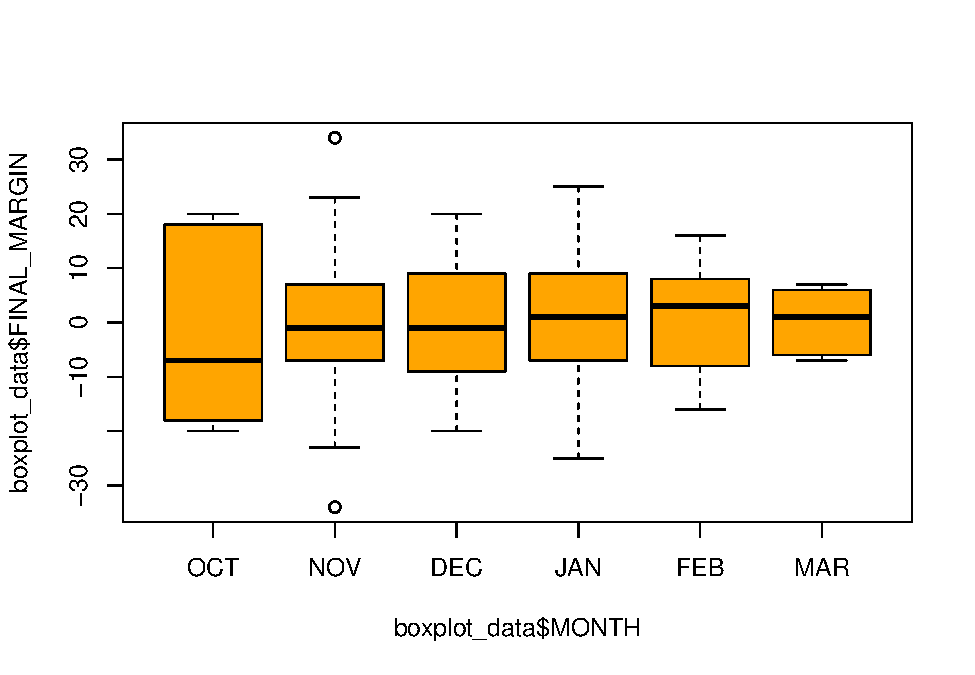
\includegraphics{index_files/figure-latex/final-margin-boxplot-1} 

}

\caption{Boxplot}\label{fig:final-margin-boxplot}
\end{figure}

The box-plot above shows how the performance of the team changed over the months. It illustrates the average margin of points the team had with the opponent team on every month of the examined period. In the first three months shown, the average final margin is being under zero with February and March appearing to be the most efficient months for the team.

\pagebreak

\begin{table}[H]

\caption{\label{tab:summary-continious-lal-data}Summary of continuous data of Los Angeles Lakers}
\centering
\begin{tabular}[t]{lccccc}
\toprule
  &  SHOT\_NUMBER &    DRIBBLES &   TOUCH\_TIME &   SHOT\_DIST &      FGM\\
\midrule
 & Min.   : 1.000 & Min.   : 0.000 & Min.   : 0.000 & Min.   : 0.10 & Min.   :0.0000\\
 & 1st Qu.: 3.000 & 1st Qu.: 0.000 & 1st Qu.: 0.900 & 1st Qu.: 5.00 & 1st Qu.:0.0000\\
 & Median : 5.000 & Median : 1.000 & Median : 1.700 & Median :15.10 & Median :0.0000\\
 & Mean   : 6.562 & Mean   : 1.986 & Mean   : 2.853 & Mean   :13.89 & Mean   :0.4544\\
 & 3rd Qu.: 9.000 & 3rd Qu.: 2.000 & 3rd Qu.: 3.800 & 3rd Qu.:22.30 & 3rd Qu.:1.0000\\
\addlinespace
 & Max.   :37.000 & Max.   :29.000 & Max.   :22.800 & Max.   :45.20 & Max.   :1.0000\\
\bottomrule
\end{tabular}
\end{table}

Table two shows the summary of some variables I considered important for predicting if a shot is going to be successful or not. It is important to mention that the \texttt{LAL} player's perform in average less than two dribbles and keep the ball just \texttt{2.85} seconds in average before shooting. An average player shots only about six times in a game and the average shot distance is \texttt{13.89} feet while most shoots are shot from \texttt{\textasciitilde{}5\ to\ \textasciitilde{}22} feet. Finally, the mean value for scores made is under 50\% as observed from the \texttt{FGM} variables which shows whether a shot is succesfuly made or not.

\begin{figure}

{\centering 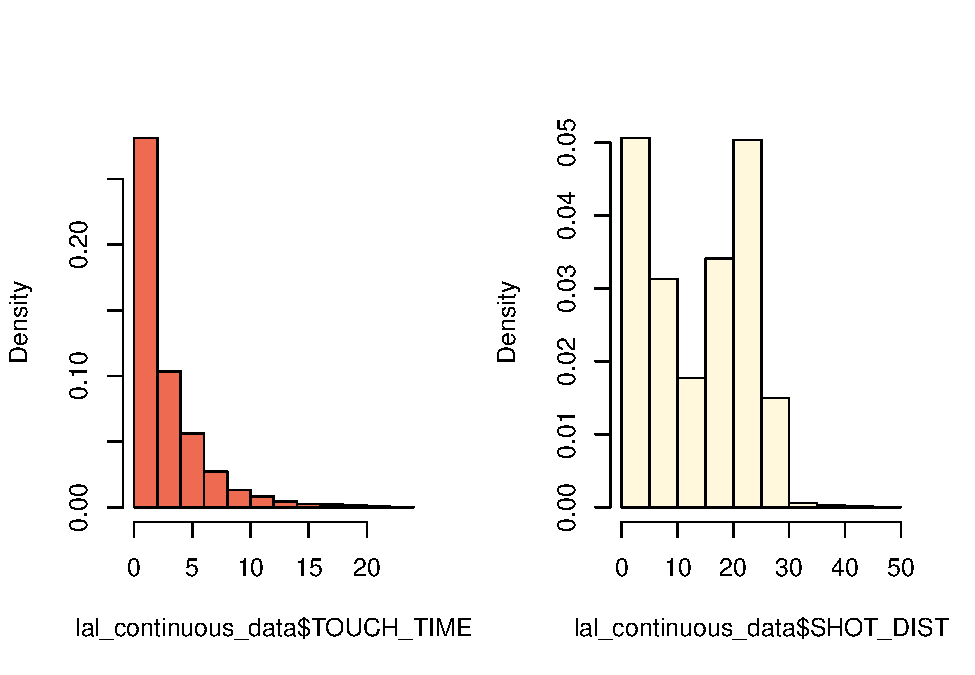
\includegraphics{index_files/figure-latex/histo-touch-time-shot-dist-1} 

}

\caption{Histograms of touch time and shot distance for the Los Angeles Lakers team.}\label{fig:histo-touch-time-shot-dist}
\end{figure}

The two histograms illustrated, do not seem to follow a normal distribution because unfortunately I do not have enough samples, although, based on what the \texttt{central\ limit\ theorem} suggests, I will assume that all the variables used in this paper are normally distributed.

\pagebreak

\hypertarget{inferential-analysis}{%
\section{Inferential Analysis}\label{inferential-analysis}}

\hypertarget{differences-between-shot-distance-for-lal-lost-games-and-min-won-games}{%
\subsection{\texorpdfstring{Differences between \texttt{shot\ distance} for \texttt{LAL\ lost\ games} and \texttt{MIN\ won\ games}}{Differences between shot distance for LAL lost games and MIN won games}}\label{differences-between-shot-distance-for-lal-lost-games-and-min-won-games}}

\begin{figure}

{\centering 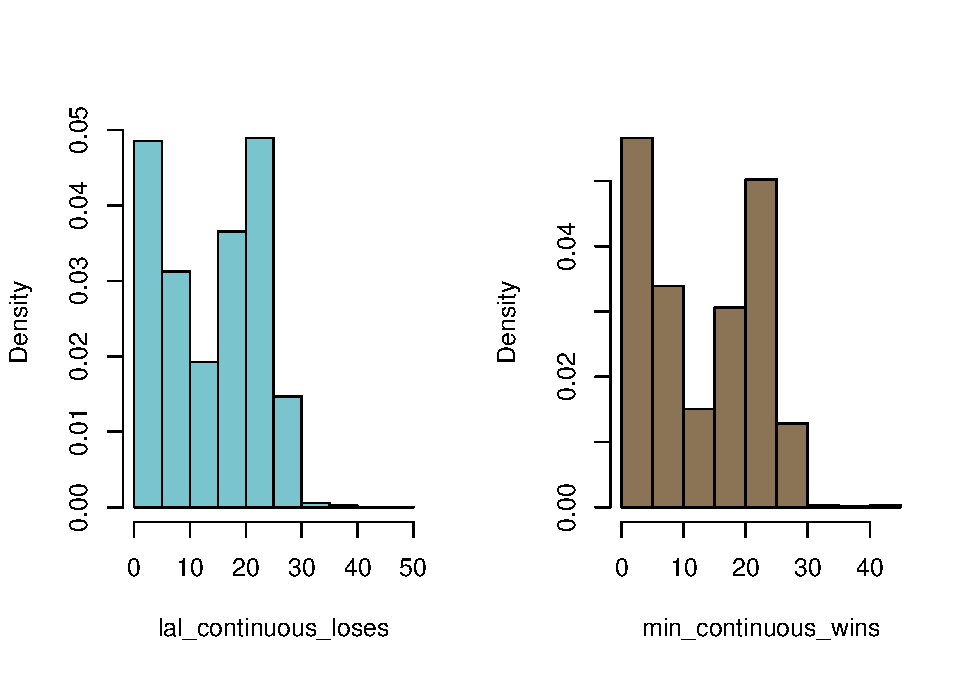
\includegraphics{index_files/figure-latex/histo-first-test-1} 

}

\caption{Histograms of lost games for LAL and won games for MIN}\label{fig:histo-first-test}
\end{figure}

\hypertarget{test-for-equality-of-varainces}{%
\subsubsection{Test for equality of varainces}\label{test-for-equality-of-varainces}}

\begin{table}[H]
\caption{\label{tab:first-var-test1}Test for equality of varainces}

\centering
\begin{tabular}[t]{ccccccc}
\toprule
estimate & num.df & den.df & statistic & p.value & conf.low & conf.high\\
\midrule
0.9334912 & 4561 & 4029 & 0.9334912 & 0.0242734 & 0.8791355 & 0.9910959\\
\bottomrule
\end{tabular}
\centering
\begin{tabular}[t]{cc}
\toprule
method & alternative\\
\midrule
F test to compare two variances & two.sided\\
\bottomrule
\end{tabular}
\end{table}

We observe that \(1\) does not belong to the confidence region at the significance level \(\alpha=0.05\), and we thus conclude that there is \textbf{not} strong statistical evidences suggesting that the variances of the shot distance during the won games of the \(MIN\) team and the lost games of the \(LAL\) team may be equal. Also, the distributions of the two samples do not seem to be Gaussian; however, the sample sizes are quite large (\(>5000\) observation for MIN, and \(>5000\) for LAL), so that the Gaussian approximation is realistic.

\begin{table}[H]
\caption{\label{tab:first-var-test2}Test for difference of varainces (LAL greater MIN)}

\centering
\begin{tabular}[t]{ccccccc}
\toprule
estimate & num.df & den.df & statistic & p.value & conf.low & conf.high\\
\midrule
0.9334912 & 4561 & 4029 & 0.9334912 & 0.9878633 & 0.8876586 & Inf\\
\bottomrule
\end{tabular}
\centering
\begin{tabular}[t]{cc}
\toprule
method & alternative\\
\midrule
F test to compare two variances & greater\\
\bottomrule
\end{tabular}
\end{table}

The previous two-sample variance tests indicates that there is very strong statistical evidences suggesting that the variance of shot distance for \texttt{LAL\ -\ loses} is larger than the one for \texttt{MIN\ -\ Wins}.

\begin{table}[H]
\caption{\label{tab:first-var-test3}Test for equality of mean}

\centering
\begin{tabular}[t]{ccccccc}
\toprule
estimate & estimate1 & estimate2 & statistic & p.value & parameter & conf.low\\
\midrule
0.6423525 & 13.95962 & 13.31727 & 3.396807 & 0.0006849 & 8379.882 & 0.2716604\\
\bottomrule
\end{tabular}
\centering
\begin{tabular}[t]{cc}
\toprule
conf.high & method\\
\midrule
1.013045 & Welch Two Sample t-test\\
\bottomrule
\end{tabular}
\end{table}

We observe that 0 does not belong to the 95\% confidence region for the var.equal=FALSE test; the obtained p-value is also relatively low. We thus conclude that there is statistical evidences suggesting that the mean shot distance of the won games of MIN could be different of the mean of the lost games of LAL.

\begin{table}[H]
\caption{\label{tab:first-var-test4}Test for difference of mean (MIN greater LAL)}

\centering
\begin{tabular}[t]{ccccccc}
\toprule
estimate & estimate1 & estimate2 & statistic & p.value & parameter & conf.low\\
\midrule
-0.6423525 & 13.31727 & 13.95962 & -3.396807 & 0.9996575 & 8379.882 & -0.9534366\\
\bottomrule
\end{tabular}
\centering
\begin{tabular}[t]{cc}
\toprule
conf.high & method\\
\midrule
Inf & Welch Two Sample t-test\\
\bottomrule
\end{tabular}
\end{table}

The test for the difference in mean indicates that the mean number of shot distance during the MIN - won games is significatly larger that the mean number of shot distance during the LAL - lost games.

From the variance and mean tests we conclude that Los Angeles Lakers, on their lost games they used to attempt to shot from shorter distance than the players of the Minnesota Timberwolves team. This could led the Timberwolves players to achieve more three-points which is maybe a more worth it to follow strategy.

\pagebreak

\hypertarget{difference-in-the-mean-touch-time-as-function-of-the-month}{%
\subsection{\texorpdfstring{Difference in the mean \texttt{touch\ time} as function of the \texttt{Month}}{Difference in the mean touch time as function of the Month}}\label{difference-in-the-mean-touch-time-as-function-of-the-month}}

\begin{figure}

{\centering 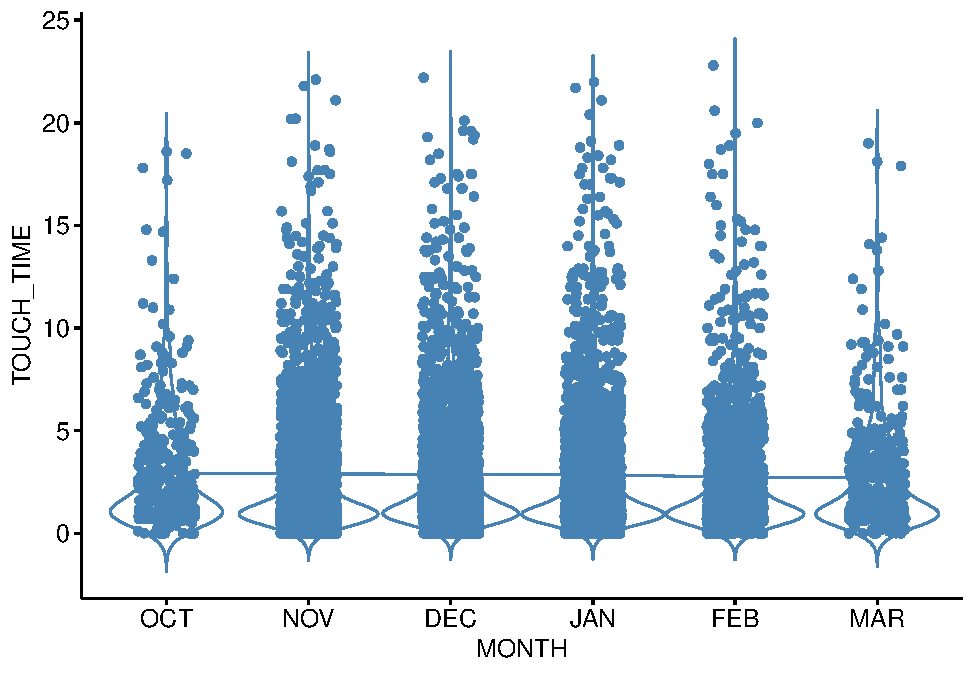
\includegraphics{index_files/figure-latex/ggline-touchtime-month-1} 

}

\caption{Plot of the touch time per month}\label{fig:ggline-touchtime-month}
\end{figure}

The touch time seems to follow a similar distribution of the samples for all the months shown.

\begin{table}[H]

\caption{\label{tab:second-test1}Fligner-Killeen test of homogeneity of variances}
\centering
\begin{tabular}[t]{cccc}
\toprule
statistic & p.value & parameter & method\\
\midrule
3.40366 & 0.6380125 & 5 & Fligner-Killeen test of homogeneity of variances\\
\bottomrule
\end{tabular}
\end{table}

\begin{table}[H]

\caption{\label{tab:second-test2}Bartlett test of homogeneity of variances}
\centering
\begin{tabular}[t]{cccc}
\toprule
statistic & p.value & parameter & method\\
\midrule
10.29799 & 0.0672189 & 5 & Bartlett test of homogeneity of variances\\
\bottomrule
\end{tabular}
\end{table}

We obtain a p-value a little larger that 0.05 , so that the variances for the touch time each month may potentially not be equal. The Fligner-Killeen test thus suggest that the month the game took place appears not to have a statistically significant effect on the variance of the touch time during the corresponding months.

\pagebreak

\begin{table}[H]

\caption{\label{tab:second-test3}Summary of the anova test on the residuals}
\centering
\begin{tabular}[t]{lccccc}
\toprule
  & Df & Sum Sq & Mean Sq & F value & Pr(>F)\\
\midrule
MONTH & 5 & 38.20394 & 7.640788 & 0.8286039 & 0.5290509\\
Residuals & 9050 & 83452.57767 & 9.221279 & NA & NA\\
\bottomrule
\end{tabular}
\end{table}

\begin{table}[H]

\caption{\label{tab:second-test4}One-way analysis of means (not assuming equal variances)}
\centering
\begin{tabular}[t]{ccccc}
\toprule
num.df & den.df & statistic & p.value & method\\
\midrule
5 & 2064.963 & 0.8668284 & 0.5025686 & One-way analysis of means (not assuming equal variances)\\
\bottomrule
\end{tabular}
\end{table}

The obtained p-values are significantly high (more than 0.5); the ANOVAs (with and without assuming equlity of variances) thus suggest that the month the game took place appears not to have a statistically significant effect on the mean touch time during the corresponding months.

\begin{figure}

{\centering 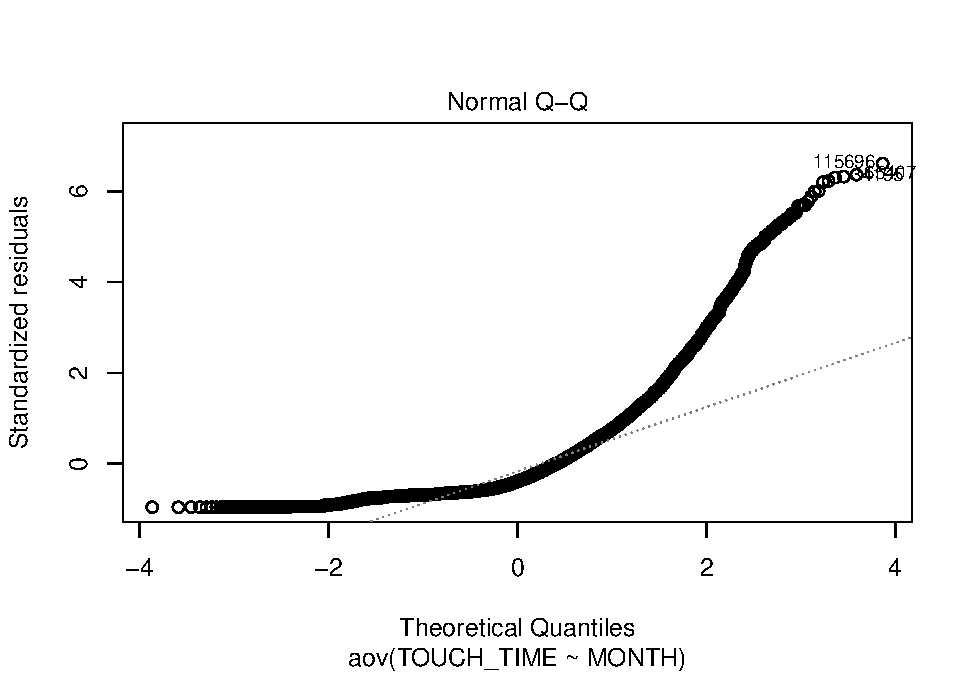
\includegraphics{index_files/figure-latex/normalqq-touchtime-month-1} 

}

\caption{Comparing two probability distributions by plotting their quantiles against each other.}\label{fig:normalqq-touchtime-month}
\end{figure}

\begin{table}[H]

\caption{\label{tab:second-test5}Shapiro-Wilk normality test}
\centering
\begin{tabular}[t]{ccc}
\toprule
statistic & p.value & method\\
\midrule
0.7564623 & 0 & Shapiro-Wilk normality test\\
\bottomrule
\end{tabular}
\end{table}

The distribution of the residuals obtained for the ANOVA res.aov1 appears significantly different from a Gaussian distribution as also shown in the \texttt{figure\ 5}. The sample size is nevertheless relatively large, so that the central limit theorem may the conclusions drawn could potentially be realistic (i.e.~the group sample mean may be close to have Gaussian distributions).

\begin{table}[H]

\caption{\label{tab:TukeyHSD-table}Tukey multiple comparison of means}
\centering
\begin{tabular}[t]{ccccccc}
\toprule
term & contrast & null.value & estimate & conf.low & conf.high & adj.p.value\\
\midrule
MONTH & MAR-DEC & 0 & -0.1728591 & -0.6326998 & 0.2869816 & 0.8928046\\
MONTH & FEB-JAN & 0 & -0.1355675 & -0.4328922 & 0.1617571 & 0.7854130\\
MONTH & MAR-JAN & 0 & -0.1663067 & -0.6298489 & 0.2972355 & 0.9105318\\
MONTH & MAR-FEB & 0 & -0.0307392 & -0.5150677 & 0.4535893 & 0.9999733\\
\bottomrule
\end{tabular}
\end{table}

The pairwise comparisons of means (95\% family-wise confidence level) suggests that there is a statistically significant difference for many pairs of months (for instance, NOV-MAR and OCT-MAR). Regarding the observations from the \emph{figure \ref{fig:final-margin-boxplot}} and the notice that the mean of the touch time that players of the Los Angeles Lakers team keep the ball before shooting on March is significantly larger compared to October and November; a consideration could be made, that the players are getting more concentrated and careful when the end of the event is closer.

\hypertarget{logistic-regression-on-successful-shot-prospect}{%
\subsection{\texorpdfstring{\texttt{Logistic\ regression} on successful shot prospect}{Logistic regression on successful shot prospect}}\label{logistic-regression-on-successful-shot-prospect}}

Predicting the probability that a shot is made successfully if variables SHOT\_DISTANCE and TOUCH\_TIME are given. This model will allow us to examine what influence the two variables have on whether a shot is successfully made or not. I ran the logistic regression model using the \texttt{FGM} as the target variable. The null hypothesis of the model is that shot distance and touch time do not influence the probability of successfully making a shot.

\begin{table}[H]

\caption{\label{tab:logistic-reg-table}Logistic regression estimators output}
\centering
\begin{tabular}[t]{lcccc}
\toprule
  & Estimate & Std. Error & z value & Pr(>|z|)\\
\midrule
(Intercept) & 0.6074778 & 0.0463442 & 13.107953 & 0\\
TOUCH\_TIME & -0.0459235 & 0.0073479 & -6.249894 & 0\\
SHOT\_DIST & -0.0480566 & 0.0025082 & -19.159974 & 0\\
\bottomrule
\end{tabular}
\end{table}

From the above table, we can observe that the \texttt{P-values} are zero; from that we can assume that the log(odds) and the log(odds ratios) are both statistically significant. Although, the effect sizes shown on the estimate column are considerably low. That means that whether a shot is made or missed, depends on the two variables examined but not in a very significant rate. Specifically, only \texttt{-0.046} for the \texttt{TOUCH\_TIME} variable and \texttt{-0.048} for the \texttt{SHOT\_DIST} variable. This means that a slight reduce on both the touch time and the shot distance from the players whenever they shoot might help the accuracy of the shot.

The reason for the effect of the variables being too small may occur by the fact that whether the shot is going to be succesfull or not is affected by many more variables and not just the two examined on this paper.

We can also calculate the Pseudo R(sqrt) which will give a more general image for this model.

\[R^2 = \text{0.0328059 - indicates the overall effect of the two examined variables.}\]

\[P-value = \text{0 - the p-value for the } R^2 \text{ using a Chi-square distribution.}\]

As expected, the R(sqrt) has a low value (low affect on the \texttt{FGM} variable), although both the variables used are being statistically significant.

\hypertarget{conclusion}{%
\section{Conclusion}\label{conclusion}}

In conclusion, as the goal of this paper is to give advice for improvement to the Los Angeles Lakers team of 2014-2015; regarding the results extracted by the inferential analysis made, we can advice the players to shoot the ball from longer distances, following the habits of one of the best teams of that period of time, Minnesota Timberwolves which gives us the suspicion that they might attempt more three-pointers than the Los Angeles team.

Another advice for the Los Angeles Lakers team could be to keep the ball longer before shooting, allowing themselves to aim better and get more steady on their feet, as this seem that affected there performance negatively during the months October and Nobember 2014.

A final conclusion, regarding the logistic regression model built during this research, is that the two variables mentioned above are affecting a shot by a very small percentage. In order to investigate more in depth the successfulness of a shot we need much more variables, even more than someone could think of.

\pagebreak

\hypertarget{appendix.}{%
\section{Appendix.}\label{appendix.}}

\begin{verbatim}
## 
## Call:
## glm(formula = IsIN ~ TOUCH_TIME + SHOT_DIST, family = binomial(link = "logit"), 
##     data = data_INxOUT)
## 
## Deviance Residuals: 
##     Min       1Q   Median       3Q      Max  
## -1.4374  -1.0495  -0.8815   1.1461   1.9182  
## 
## Coefficients:
##              Estimate Std. Error z value Pr(>|z|)    
## (Intercept)  0.607478   0.046344   13.11  < 2e-16 ***
## TOUCH_TIME  -0.045923   0.007348   -6.25 4.11e-10 ***
## SHOT_DIST   -0.048057   0.002508  -19.16  < 2e-16 ***
## ---
## Signif. codes:  0 '***' 0.001 '**' 0.01 '*' 0.05 '.' 0.1 ' ' 1
## 
## (Dispersion parameter for binomial family taken to be 1)
## 
##     Null deviance: 12479  on 9055  degrees of freedom
## Residual deviance: 12069  on 9053  degrees of freedom
## AIC: 12075
## 
## Number of Fisher Scoring iterations: 4
\end{verbatim}

  \bibliography{refs.bib}

\end{document}
